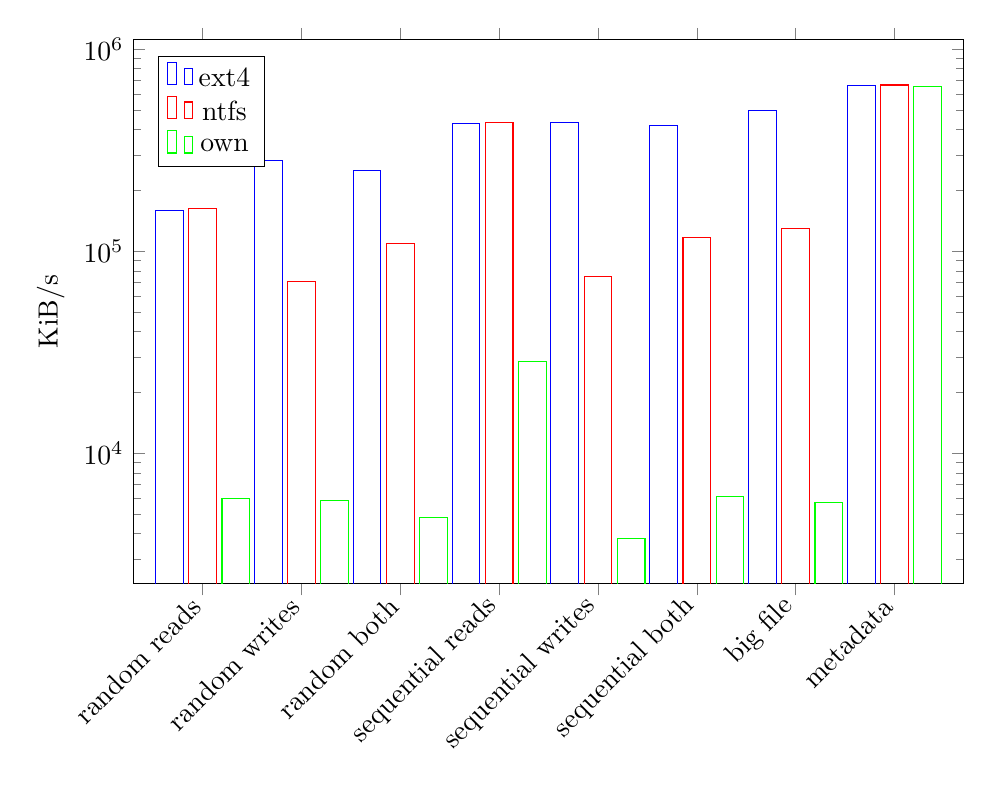
\begin{tikzpicture}
\begin{axis} [
    % TODO: add labels on data (useful)
    ybar, ymode = log,
    ylabel = {KiB/s},
    % nodes near coords,
    % nodes near coords align = {vertical},
    % enlargelimits=0.1,
    width=\textwidth, height = 0.7\textwidth,
    symbolic x coords = {
        random reads, random writes, random both,
        sequential reads, sequential writes, sequential both,
        big file, metadata
    },
    x tick label style = {rotate = 45, anchor = east},
    legend pos = {north west}
]

    % ext
    \addplot[
        draw=blue
    ] coordinates {
        (random reads, 159403) (random writes, 280917) (random both, 250539)
        (sequential reads, 430421) (sequential writes, 432469) (sequential both, 417792)
        (big file, 497323) (metadata, 663893)
    };

    % ntfs
    \addplot[
        draw=red
    ] coordinates {
        (random reads, 162133) (random writes, 70519) (random both, 109670)
        (sequential reads, 431445) (sequential writes, 74684) (sequential both, 116395)
        (big file, 128956) (metadata, 664576)
    };

    % own
    \addplot[
        draw=green
    ] coordinates {
        (random reads, 5963) (random writes, 5812) (random both, 4820)
        (sequential reads, 28331) (sequential writes, 3799) (sequential both, 6104)
        (big file, 5693) (metadata, 651947)
    };

    \legend{ext4, ntfs, own};

\end{axis}
\end{tikzpicture}
